\chapter{Tokamak Concept}
\label{chap:TokamakConcept}
Fusion reactions require extreme temperatures at about 15keV to happen. At such high temperatures, any matter transforms into an ionized state, called plasma, where electrons are dissociated from their atomic core. Charged particles are particularly responsive to magnetic fields, a property that will be used by tokamaks to confine the hot plasma and protect the physical walls of the device. 

A deuterium plasma is an ionized gas comprising positively charged ions ($D^+$) and negatively charged electrons ($e^-$). Initially, both species exhibit independent dynamics. Despite having exactly opposite charges, ions are significantly heavier than electrons, with a mass ratio of $m_i/m_e \approx 3.7\cdot 10^3$. Both ions and electrons can be described by their respective momenta and temperatures. In Sec. \ref{sec:intro_particlesInPlasma}, we first describe their independent behavior in a magnetized environment, then how species interact in Sec. \ref{sec:intro_particlesInteration} and we finish with Sec. \ref{sec:intro_SOL} about the importance of the Scrape-Off-Layer.


\section{Particles in a magnetized plasma}
\label{sec:intro_particlesInPlasma}
This first section is dedicated to elucidate the fundamental working principle of tokamaks. Before all, we must understand how charged particles behave when exposed to strong magnetic fields (in Sec. \ref{ssec:intro_magneticConfinement}) and how this knowledge allows us to design a magnetic "cage", in which particles are trapped, or confined (in Sec. \ref{ssec:intro_tokamakConfiguration}). The governing equations of this magnetic configuration are given in Sec. \ref{sec:intro_GradShafranov} and Sec. \ref{ssec:intro_limitedDivertedConfig} introduces and compares limited and diverted configurations.

\subsection{Magnetic confinement}
\label{ssec:intro_magneticConfinement}
To understand how charged plasma particles can be confined on a magnetic field line, we consider the simplest example of a single particle with charge \( q \) in a homogeneous, unidirectional magnetic field \(\textbf{B}\) with directional unit vector \(\textbf{b}\). The amplitude of the magnetic field is then $B$ such that $\mathbf{B} = B\mathbf{b}$. Solely the magnetic component of Lorentz's force acts on a particle with mass \( m \) and charge \( q \), leading to the following equation for its velocity \(\textbf{v}\):

\begin{equation}
	\label{eq:gyromotion_LorentzForce}
	m\dv{\textbf{v}}{t} = q\textbf{v}\cross\textbf{B}
\end{equation}

To solve this differential equation, it is convenient to decompose the velocity vector into a parallel component \( v_\parallel = \textbf{v}\cdot\textbf{b} \) and a perpendicular component \( \textbf{v}_\perp = \textbf{v} - v_\parallel \textbf{b} \). For a given initial velocity \(\mathbf{v}_0\), the general solution of this system is:

\begin{equation}
	\mathbf{v}(t) = v_{\parallel,0}\mathbf{b} + \mathbf{v}_{\perp,0}\cos(\omega_B t) + \mathbf{b} \times \mathbf{v}_{\perp,0} \sin(\omega_B t)
\end{equation}

with \(\omega_B = \frac{qB}{m}\) being the cyclotron frequency. This implies that a charged particle circles around a magnetic field line while following it with its initial velocity. The opposite charges of ions and electrons result in them circling in different directions. The trajectory is qualitatively shown in Fig. \ref{fig:TokamakBasics_gyromotion}. The radius of this gyromotion is called the Larmor radius \(\rho_L\):

\begin{equation}
	\rho_L = \frac{m\norm{\mathbf{v}_{\perp,0}}}{qB}
\end{equation}

Because of the high mass ratio, ions have a much larger Larmor radius than electrons. This gyromotion is the fundamental mechanism behind magnetic confinement. \newline 


\begin{figure}[H]
	\centering
	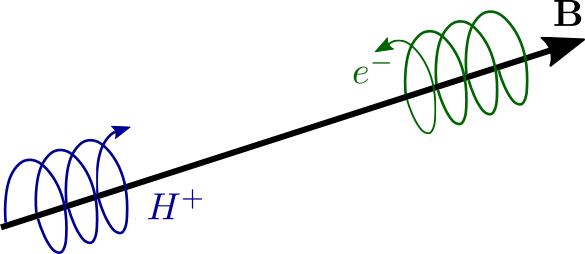
\includegraphics[width=0.62\textwidth]{schemes/gyromotion.png}
	\caption{Trajectory of a positively and a negatively charged particle along a homogeneous magnetic field line.}
	\label{fig:TokamakBasics_gyromotion}
\end{figure}


For a non-homogeneous field, Eq. \ref{eq:gyromotion_LorentzForce} does not necessarily have a straightforward solution. To assume gyromotion as the fundamental dynamic for particles, the magnetic field must remain relatively constant along the helical path traced by the field lines. This requirement imposes a criterion on the Larmor radius, known as adiabatic theory:
\begin{equation}
	\label{eq:intro_adiabaticCondition}
	\rho_L \ll \frac{B}{\norm{\grad B}}
\end{equation}


\subsection{Tokamak configuration}
\label{ssec:intro_tokamakConfiguration}
Maxwell's law stipulates that the magnetic field must be divergence-free, \(\grad\cdot\mathbf{B} = 0\). Since constructing an infinitely long machine is impractical, particle confinement requires that a given field line be closed, meaning that following its path would return one to the initial position. This necessitates some bending of the magnetic field lines. \newline
The fundamental principle of a tokamak lies in its magnetic configuration, which is designed to confine hot plasma within a toroidal chamber. This configuration comprises two primary magnetic field components: the toroidal field \( B_\varphi \) and the poloidal field \( B_p \). Coils encircling the torus generate the toroidal field, which runs parallel to the circular path of the tokamak and serves to confine the plasma. A strong current passing through the plasma itself induces the poloidal field. The combination of these fields creates a twisted, helical magnetic field structure, as shown in Fig. \ref{fig:1_magneticConfigurationTorus}, that stabilizes the plasma and helps maintain its shape and position within the tokamak.


\begin{figure}[H]
	\centering
	\begin{subfigure}[b]{0.4\textwidth}
		\centering
		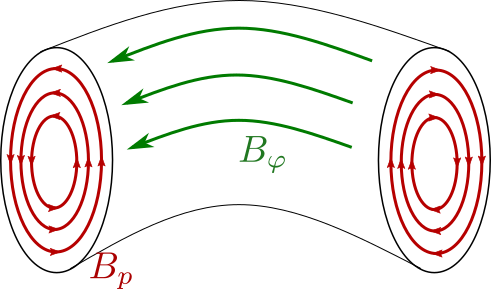
\includegraphics[width=1.\textwidth]{schemes/BpolBtor.png}
		\subcaption{Poloidal and toroidal fields}
		\label{fig:TokamakBasics_BpolBtor}
	\end{subfigure}
	\begin{subfigure}[b]{0.4\textwidth}
		\centering
		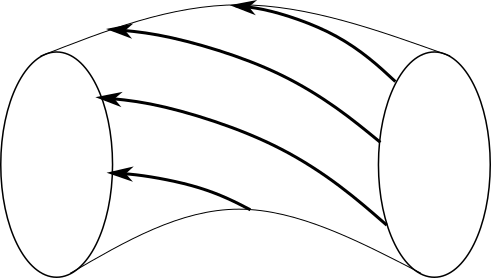
\includegraphics[width=1.\textwidth]{schemes/Btot.png}
		\subcaption{Resulting helical magnetic field}
		\label{fig:TokamakBasics_Btot}
	\end{subfigure}
	\caption{Simplified scheme of the magnetic field components on a flux surface (a) and the total magnetic field (b).}
	\label{fig:1_magneticConfigurationTorus}
\end{figure}

The helical configuration of a magnetic field line in a tokamak ensures that tracing its path remains within the same toroidal surface, ultimately returning to the initial point and forming a closed field line. The ensemble of all such field lines constitutes what is termed a "closed magnetic flux surface." These flux surfaces are radially concentric, and the principle of magnetic confinement is to trap plasma particles within these flux surfaces.\newline

At first glance, the toroidal field appears sufficient to close magnetic field lines. However, internal and external perturbations can cause twisting of the magnetic field lines, potentially leading to disruptions and total loss of plasma confinement. This phenomenon is known as kink instabilities. To suppress them, the poloidal field introduces magnetic shear to the configuration, with field lines circling around the minor radius of the torus. The ratio of toroidal to poloidal rotations of the field lines is known as the safety factor \( q = \frac{aB_\varphi}{RB_p} \). In a cylindrical approximation, the Kruskal-Shafranov limit \cite{shafranov1956stability, kruskal1958instability} states that kink instabilities are suppressed for \( q > 1 \). However, the safety factor cannot be too large either, as other instabilities such as tearing \cite{furth1973tearing} or resistive wall \cite{fitzpatrick2002simple} modes might appear and deteriorate plasma confinement. \\


\subsection{Grad-Shafranov equilibrium}
\label{sec:intro_GradShafranov}

How can the magnetic configuration be described in a more mathematical way? The magnetic configuration of a tokamak can be described mathematically in cylindrical coordinates \( (R,Z,\varphi) \) with the corresponding basis vectors \([\mathbf{e}_R,\mathbf{e}_Z,\mathbf{e}_\varphi]\). The magnetic field consists of two main components: the poloidal field \(\mathbf{B}_p\), which lies in the \((R,Z)\) plane (referred to as the "poloidal plane"), and the toroidal field \(\mathbf{B}_\varphi\), which is aligned along the \(\varphi\)-direction.

Each magnetic field \(\mathbf{B}\) is associated with a vector potential \(\mathbf{A}\) such that:

\begin{equation}
	\label{eq:intro_magneticVectorPotential}
	\nabla \times \mathbf{A} = \mathbf{B}
\end{equation}

Assuming axisymmetry, gradients along the \(\varphi\)-direction vanish. Let \(\mathbf{A} = A_R \mathbf{e}_R + A_Z \mathbf{e}_Z + A_\varphi \mathbf{e}_\varphi\) represent the three components of the vector potential. The magnetic field can then be expressed as:

\begin{equation}
	\mathbf{B} = \left(\frac{1}{R}\pdv{(RA_\varphi)}{Z}\right)\mathbf{e}_R - \left(\frac{1}{R}\pdv{(RA_\varphi)}{R}\right)\mathbf{e}_Z + \left(\pdv{A_Z}{R} - \pdv{A_R}{Z}\right)\mathbf{e}_\varphi
\end{equation}

Introducing the poloidal flux function \(\Psi = -RA_\varphi\), which shapes \(\mathbf{B}_p\), and the toroidal field function \(F = RB_\varphi\), the magnetic field components can be written as:

\begin{equation}
	\label{eq:intro_BeqMagneticFluxes}
	\mathbf{B} = \underbrace{\nabla \Psi \times \nabla \varphi}_{\mathbf{B}_p} + \underbrace{F \nabla \varphi}_{\mathbf{B}_\varphi}
\end{equation}

In a tokamak, the plasma is not uniform, leading to a pressure gradient from the colder edge to the hotter core. In a stationary plasma that has reached magnetohydrodynamic (MHD) equilibrium, the magnetic and pressure forces must balance, which is described by the force balance equation:

\begin{equation}
	\nabla p = \mathbf{j} \times \mathbf{B}
\end{equation}

Because of the cross-product, $\nabla p$ is always perpendicular to $\mathbf{B}$, implying that $p$ must be constant along a field line. Under the assumption of axisymmetry, $\partial_\varphi p = 0$, meaning that the toroidal component of the magnetic force must be zero. Consequently, only the poloidal field $\mathbf{B}_p$ responds to a pressure gradient. Since the pressure $p(\Psi)$ is both axisymmetric and field-aligned, it can only be a function of the poloidal flux $\Psi$. The toroidal component of the current density can be expressed as:

\begin{equation}
	j_\varphi = R\frac{dp}{d\Psi} + \frac{F}{\mu_0 R}\frac{dF}{d\Psi}
\end{equation}

Ampère's law relates the current density $\mathbf{j}$ to the magnetic field $\mathbf{B}$, with the vacuum permeability $\mu_0$:

\begin{equation}
	\mu_0\mathbf{j} = \nabla \times \mathbf{B}
\end{equation}

This gives an alternative expression for the toroidal current:

\begin{equation}
	j_\varphi = \frac{1}{\mu_0}\left[\partial_R\left(\frac{1}{R}\partial_R\Psi\right) + \frac{1}{R}\partial_Z^2\Psi\right]
\end{equation}

By equating both expressions for $j_\varphi$, we arrive at the Grad-Shafranov equation\cite{grad1958hydromagnetic,shafranov1957equilibrium} for the poloidal flux:

\begin{equation}
	\label{eq:intro_GradShafranovEquation}
	\Delta^* \Psi = R\partial_R\left(\frac{1}{R}\partial_R\Psi\right) + \partial_Z^2\Psi = -\mu_0R^2\frac{dp}{d\Psi} - \mu_0 F \frac{dF}{d\Psi}
\end{equation}
Here we introduced the Shafranov operator $\Delta^*$.
This equation is a second-order nonlinear partial differential equation. The procedure outlined in Appendix \ref{sec:app_GradShafranovSolver} solves Eq. \ref{eq:intro_GradShafranovEquation} iteratively using a Newton-Krylov method. A typical solution for $\Psi$ is illustrated in Fig. \ref{fig:1_PsiFlux}.

\begin{figure}[H]
	\centering
	\begin{subfigure}[b]{0.45\textwidth}
		\centering
		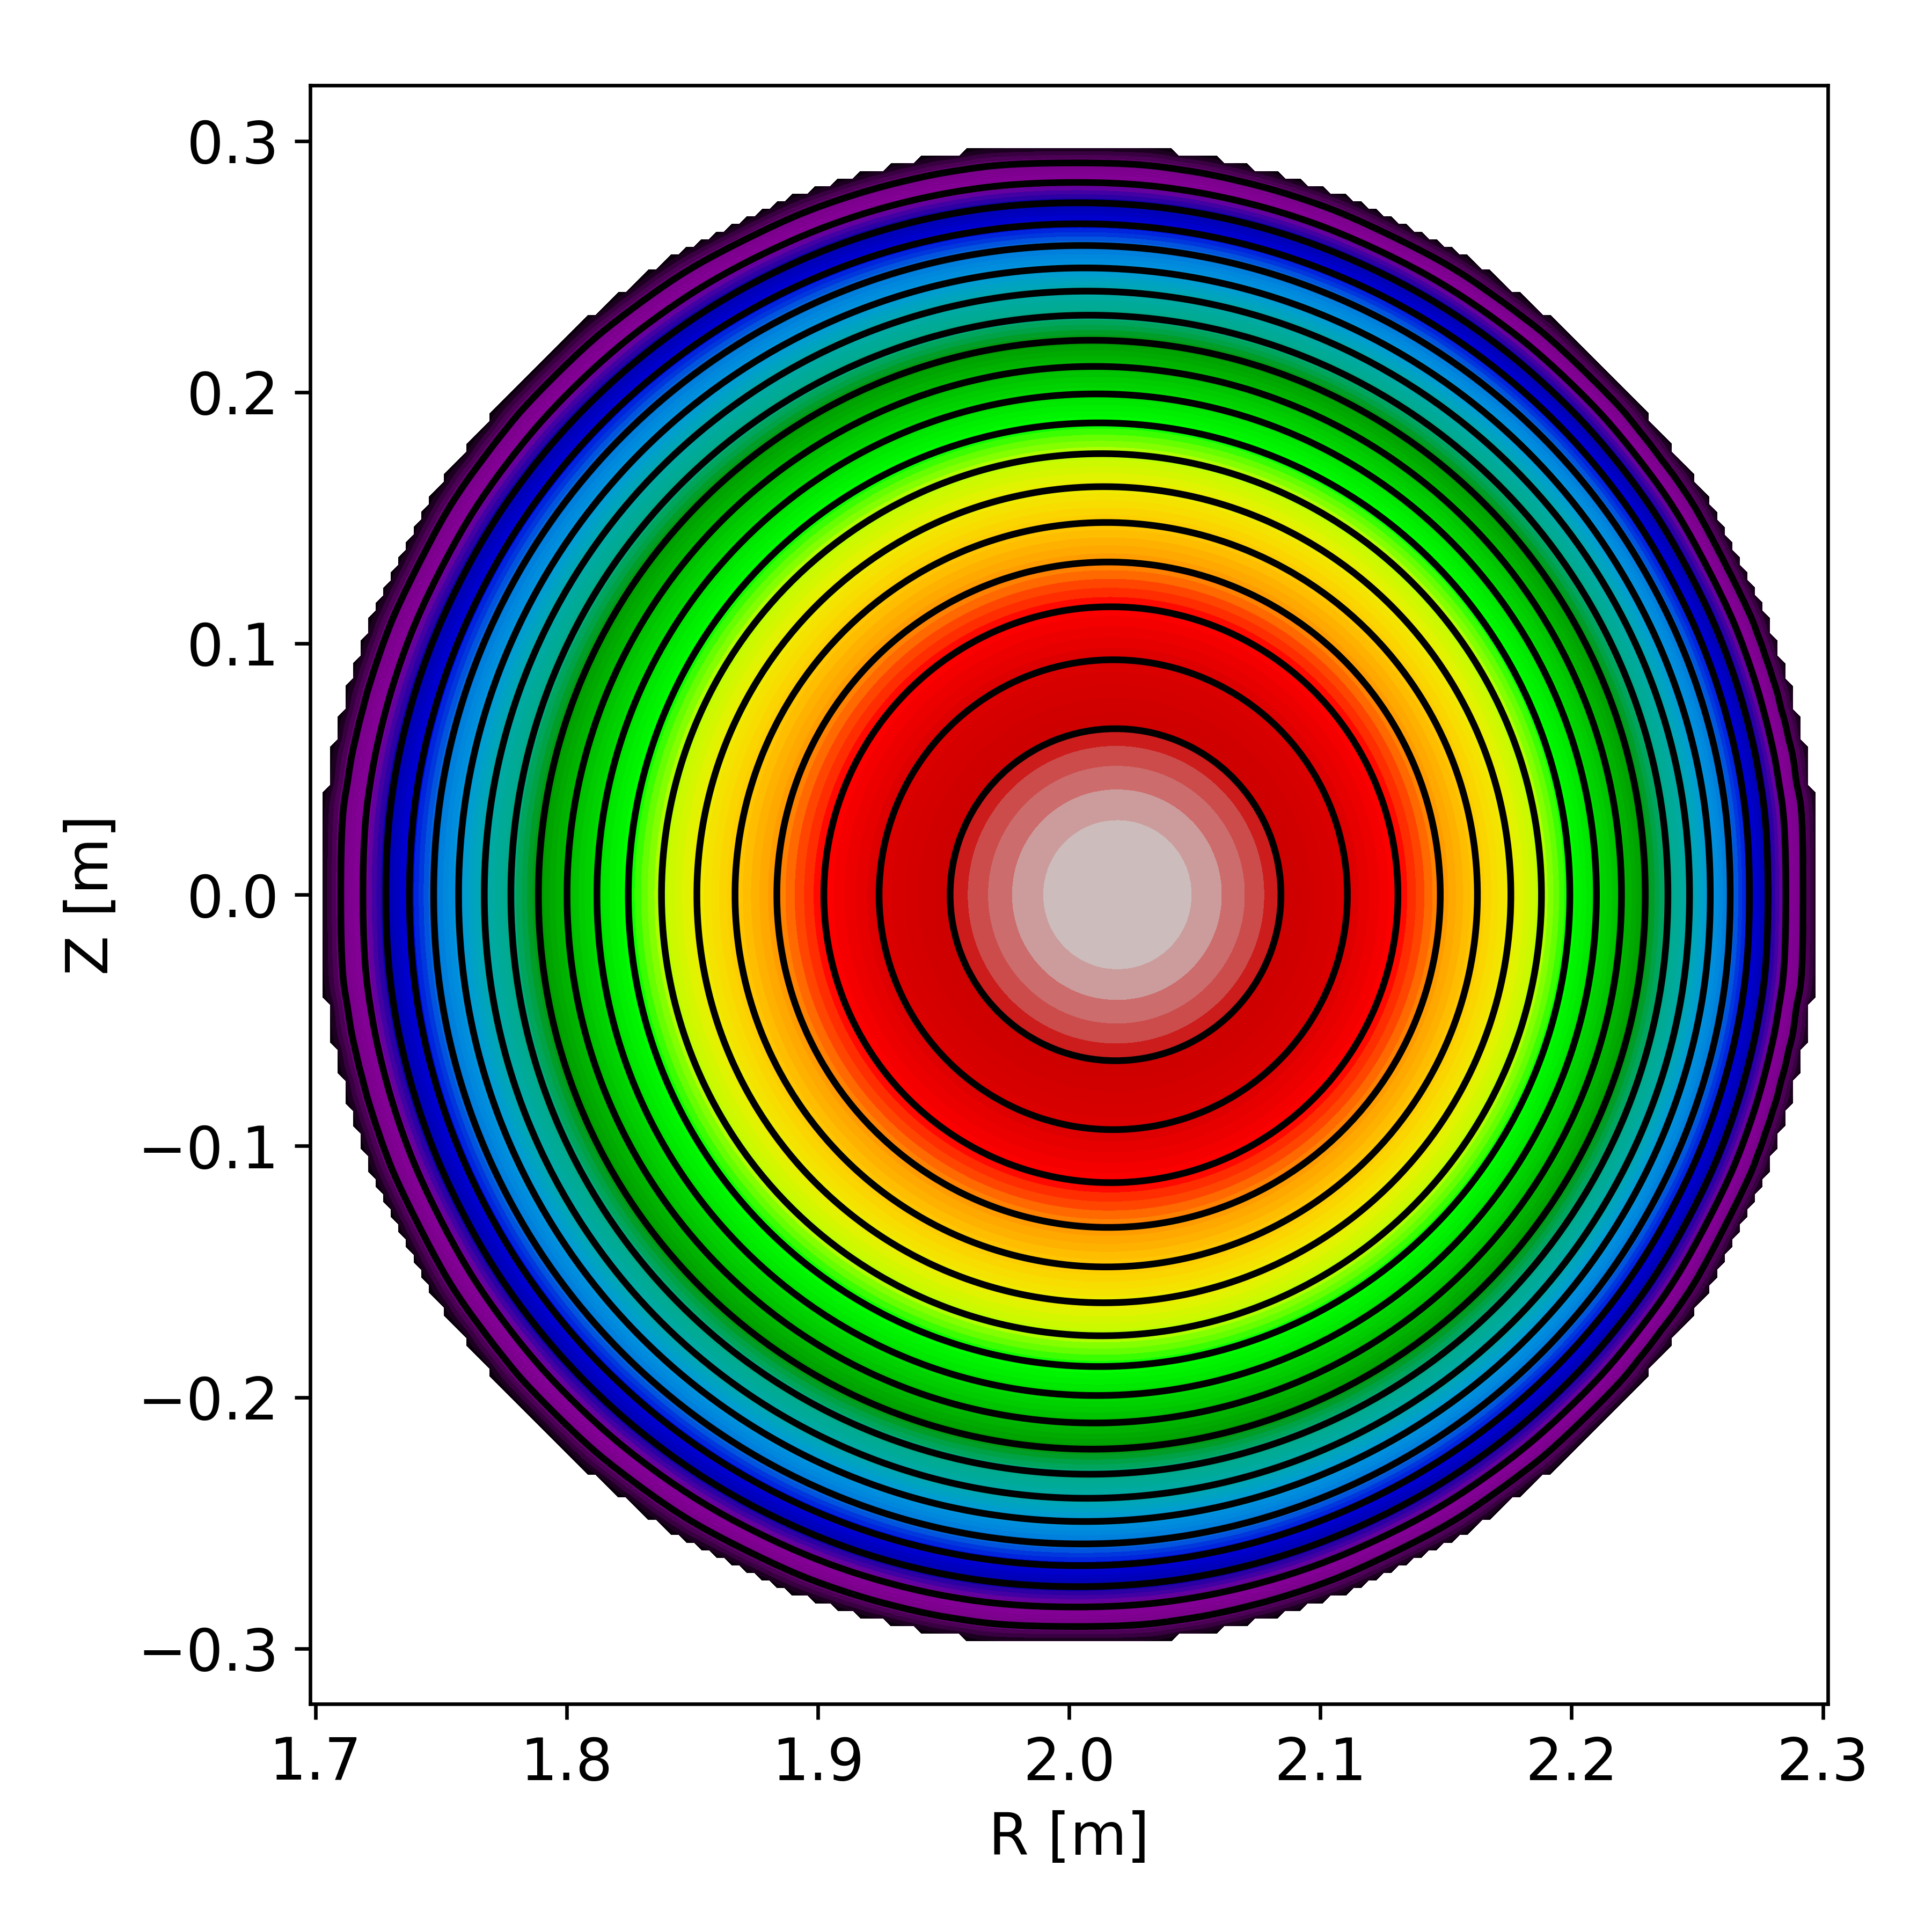
\includegraphics[height=60mm]{schemes/Psi_GradShafranov_R_2.png}
		\subcaption{Major radius $R_0 = 2$m}
		\label{fig:GS_PSI_R_2}
	\end{subfigure}
	\begin{subfigure}[b]{0.45\textwidth}
		\centering
		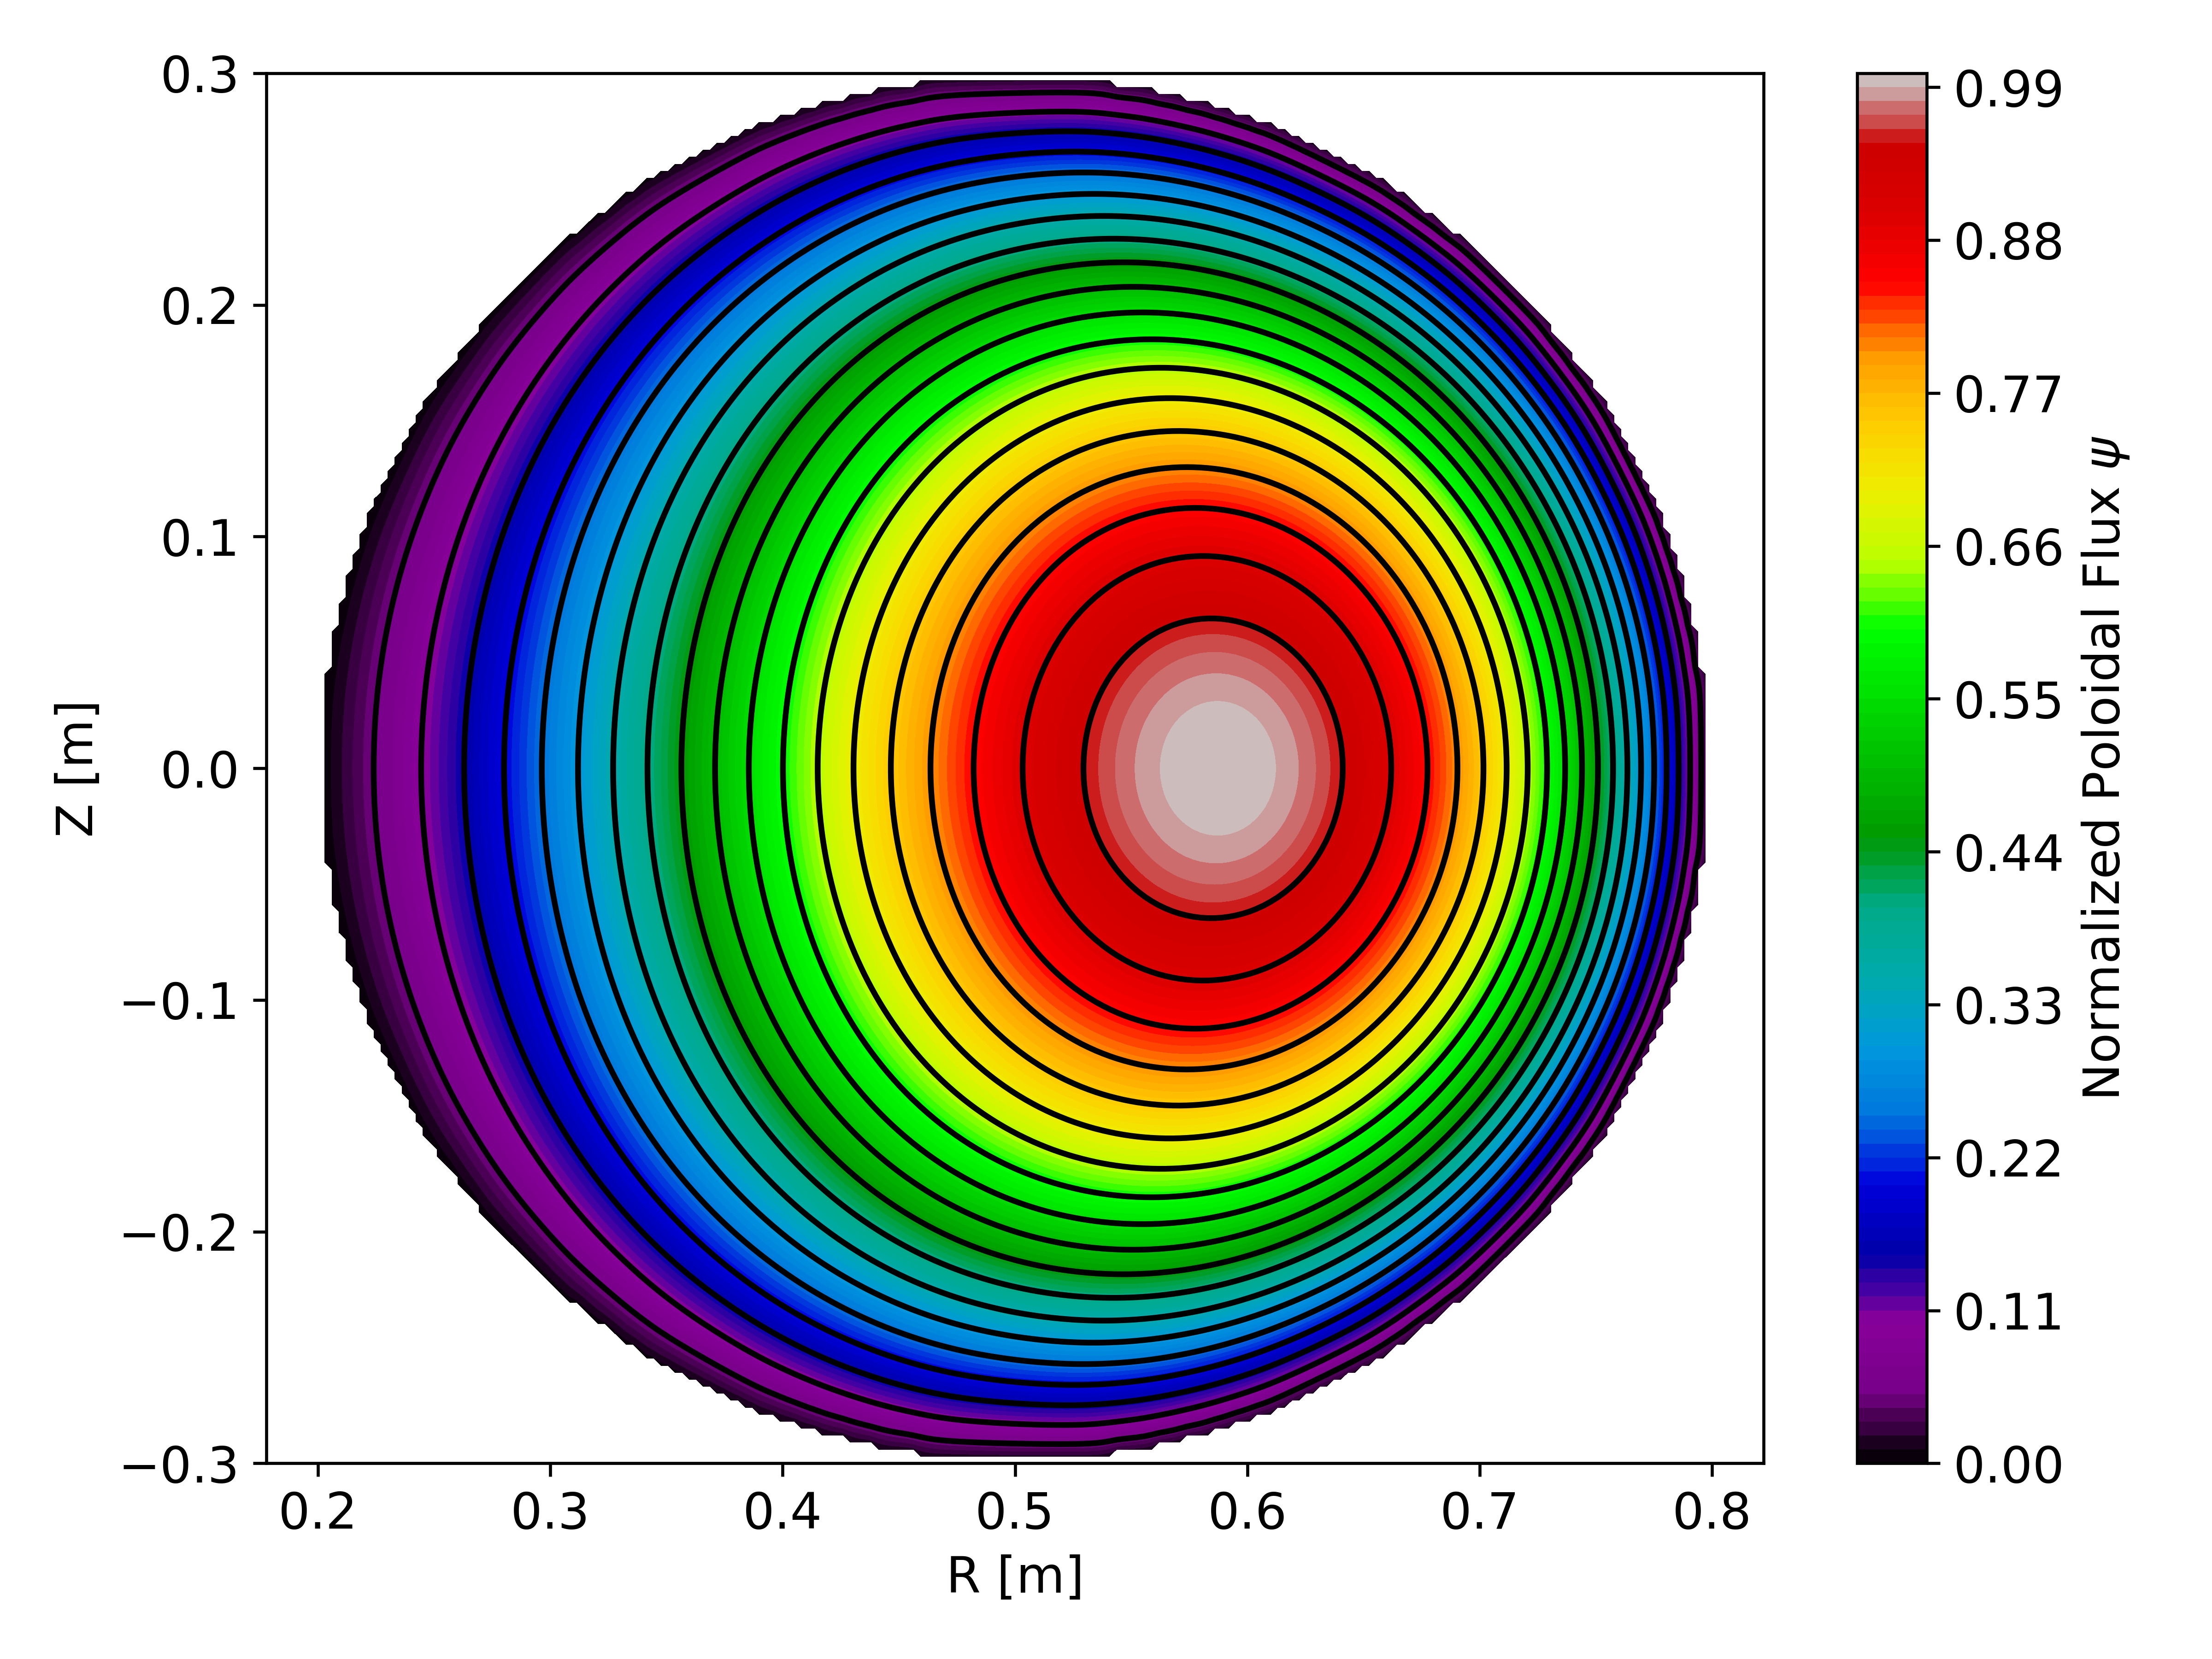
\includegraphics[height=60mm]{schemes/Psi_GradShafranov_R_0_5.png}
		\subcaption{Major radius $R_0 = 0.5$m}
		\label{fig:GS_PSI_R_0_5}
	\end{subfigure}
	\caption{Solution of the Grad-Shafranov equation on a circular cross-section with minor radius $a = 0.3$ m. A Cartesian mesh with $N = 200$ equidistant discretization points is used for the $R$ and $Z$ coordinates. The flux $\Psi$ is forced to 0 at the boundary. The toroidal magnetic field is given by $B_\varphi = B_0 R_0 / R$ with $B_0 = 1$T. The pressure follows an exponential distribution $p(\Psi) = p_0 (e^{-\Psi} - 1)$ with $p_0 = 1$ MPa.}
	\label{fig:1_PsiFlux}
\end{figure}

The plasma pressure causes the magnetic axis to shift outward in a phenomenon known as the Grad-Shafranov shift. The radial displacement from the centerline of the torus can be approximated by:

\begin{equation}
	\label{eq:intro_GradShafranovShift}
	\Delta \approx \frac{2\mu_0 p}{B_p}\frac{a^2}{R_0}
\end{equation}

The two scenarios presented in Fig. \ref{fig:1_PsiFlux} differ by their major radius. As the Grad-Shafranov shift is inversely proportional to $R_0$, we expect that the larger curvature in the case \ref{fig:GS_PSI_R_0_5} $R_0 = 0.5$m induces a larger shift, which is precisely what is observed.



\subsection{Realisation of magnetic configurations}
\label{ssec:intro_limitedDivertedConfig}

The magnetic tokamak configuration in a tokamak is controlled by a set of coils. An example of the technical realisation in the ITER tokamak is shown in Fig. \ref{1_ITER}. The fundamental configuration discussed before, is created by the toroidal field coils encircling the plasma chamber, appear in orange on the scheme. As it  from the name, they drive the toroidal magnetic field $B_\varphi$. The poloidal field, necessary for the helical path of confined plasma particles, is driven by a strong toroidal current, itself induced by the central solenoid (central column with yellow ends). 

They are completed by poloidal field coils (light purple), placed outside the main plasma chamber and distributed along the height of the tokamak. They generate a poloidal magnetic field that wraps around the plasma with the minor radius, perpendicular to the toroidal field. By adjusting the current, it is possible to control the vertical position, elongation, and triangularity of the plasma. For example, increasing the current in certain poloidal coils can elongate the plasma, giving it an oval cross-section, or induce triangularity by pulling the plasma boundary inward at the top and bottom. 

\begin{figure}[H]
	\centering
	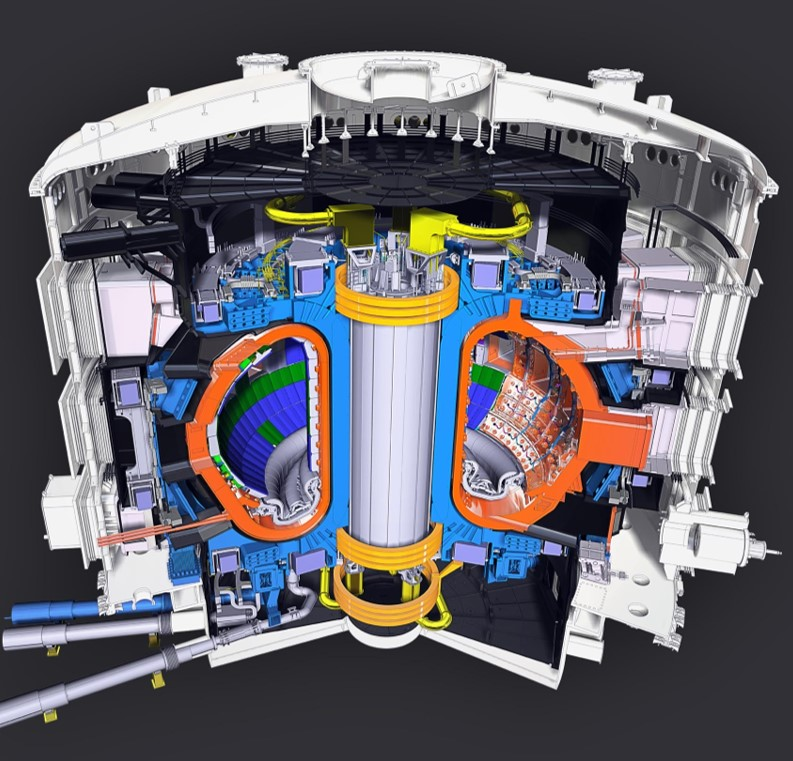
\includegraphics[width=0.8\textwidth]{schemes/ITER_2.jpg}
	\caption{Cutaway of the ITER tokamak (source: ITER Organization)}
	\label{fig:1_ITER}
\end{figure}

The limited configuration is one of the simpler magnetic configurations in a tokamak. In this setup, the plasma is in direct contact with material components which act as a limiter (see Fig. \ref{fig:WEST_limited}). The confined plasma boundary is given by the last closed flux surface, tangential to the wall in one point. Such a configuration suffers from significant power loads on the limiters, resulting in high erosion rates and potential contamination of the plasma with impurities. The confinement is generally lower in this configuration.

A diverted configuration, as depicted in Fig. \ref{fig:WEST_diverted}, improves the situation by a lot. The poloidal field coils shape the magnetic field lines in a fashion that they do not intersect with solid surfaces within the main plasma chamber but are instead directed to a separate region called the divertor. The last closed flux surface is then called "separatrix" and never touches the tokamak wall. It effectively splits the domain in a confined core region with closed field lines and the Scrape-Off-Layer (SOL), that extends to the wall and where field lines are open, e.g. they cross the wall. The poloidal magnetic field contains now a singularity, the "X-point", and the area where the he divertor plate intecepts the continuation of the separatrix is called the "target line". The divertor handles the exhaust of heat and particles from the plasma and this configuration tends to improve overall plasma confinement and reduce impurity levels.

\begin{figure}[H]
	\centering
	\begin{subfigure}[b]{0.45\textwidth}
		\centering
		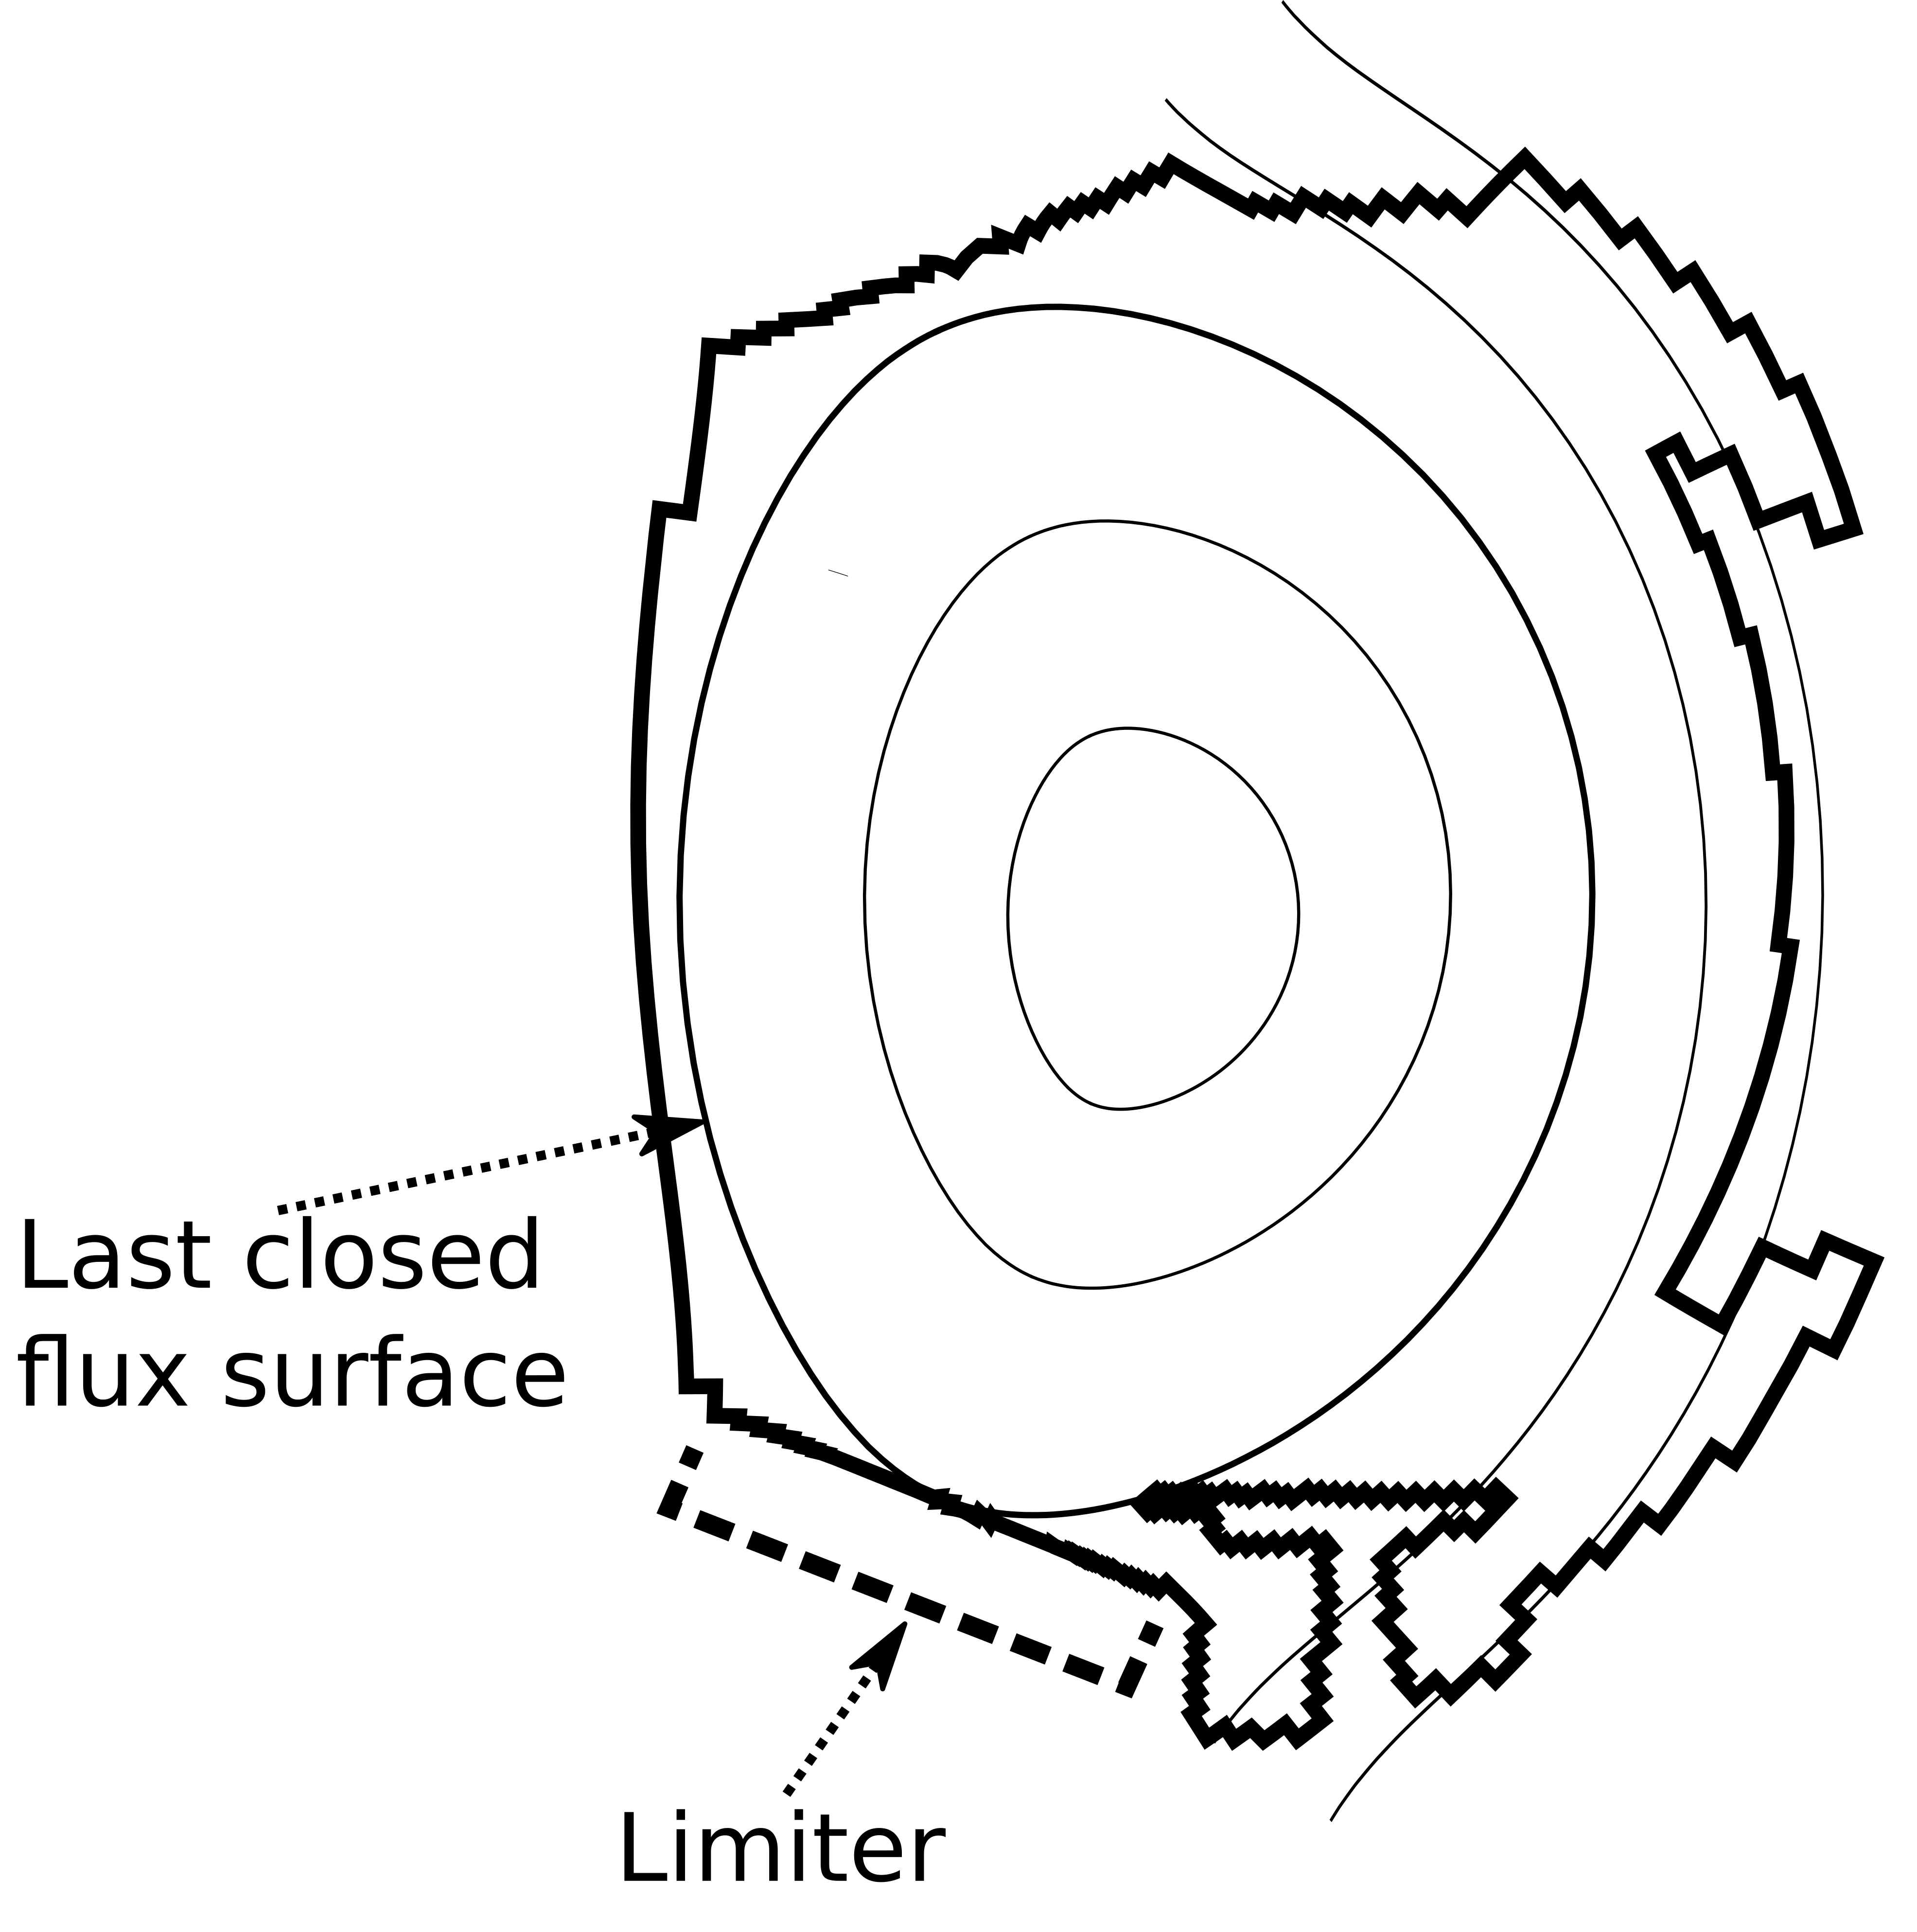
\includegraphics[height=60mm]{schemes/WESTlimited.png}
		\subcaption{Limited configuration}
		\label{fig:WEST_limited}
	\end{subfigure}
	\begin{subfigure}[b]{0.45\textwidth}
		\centering
		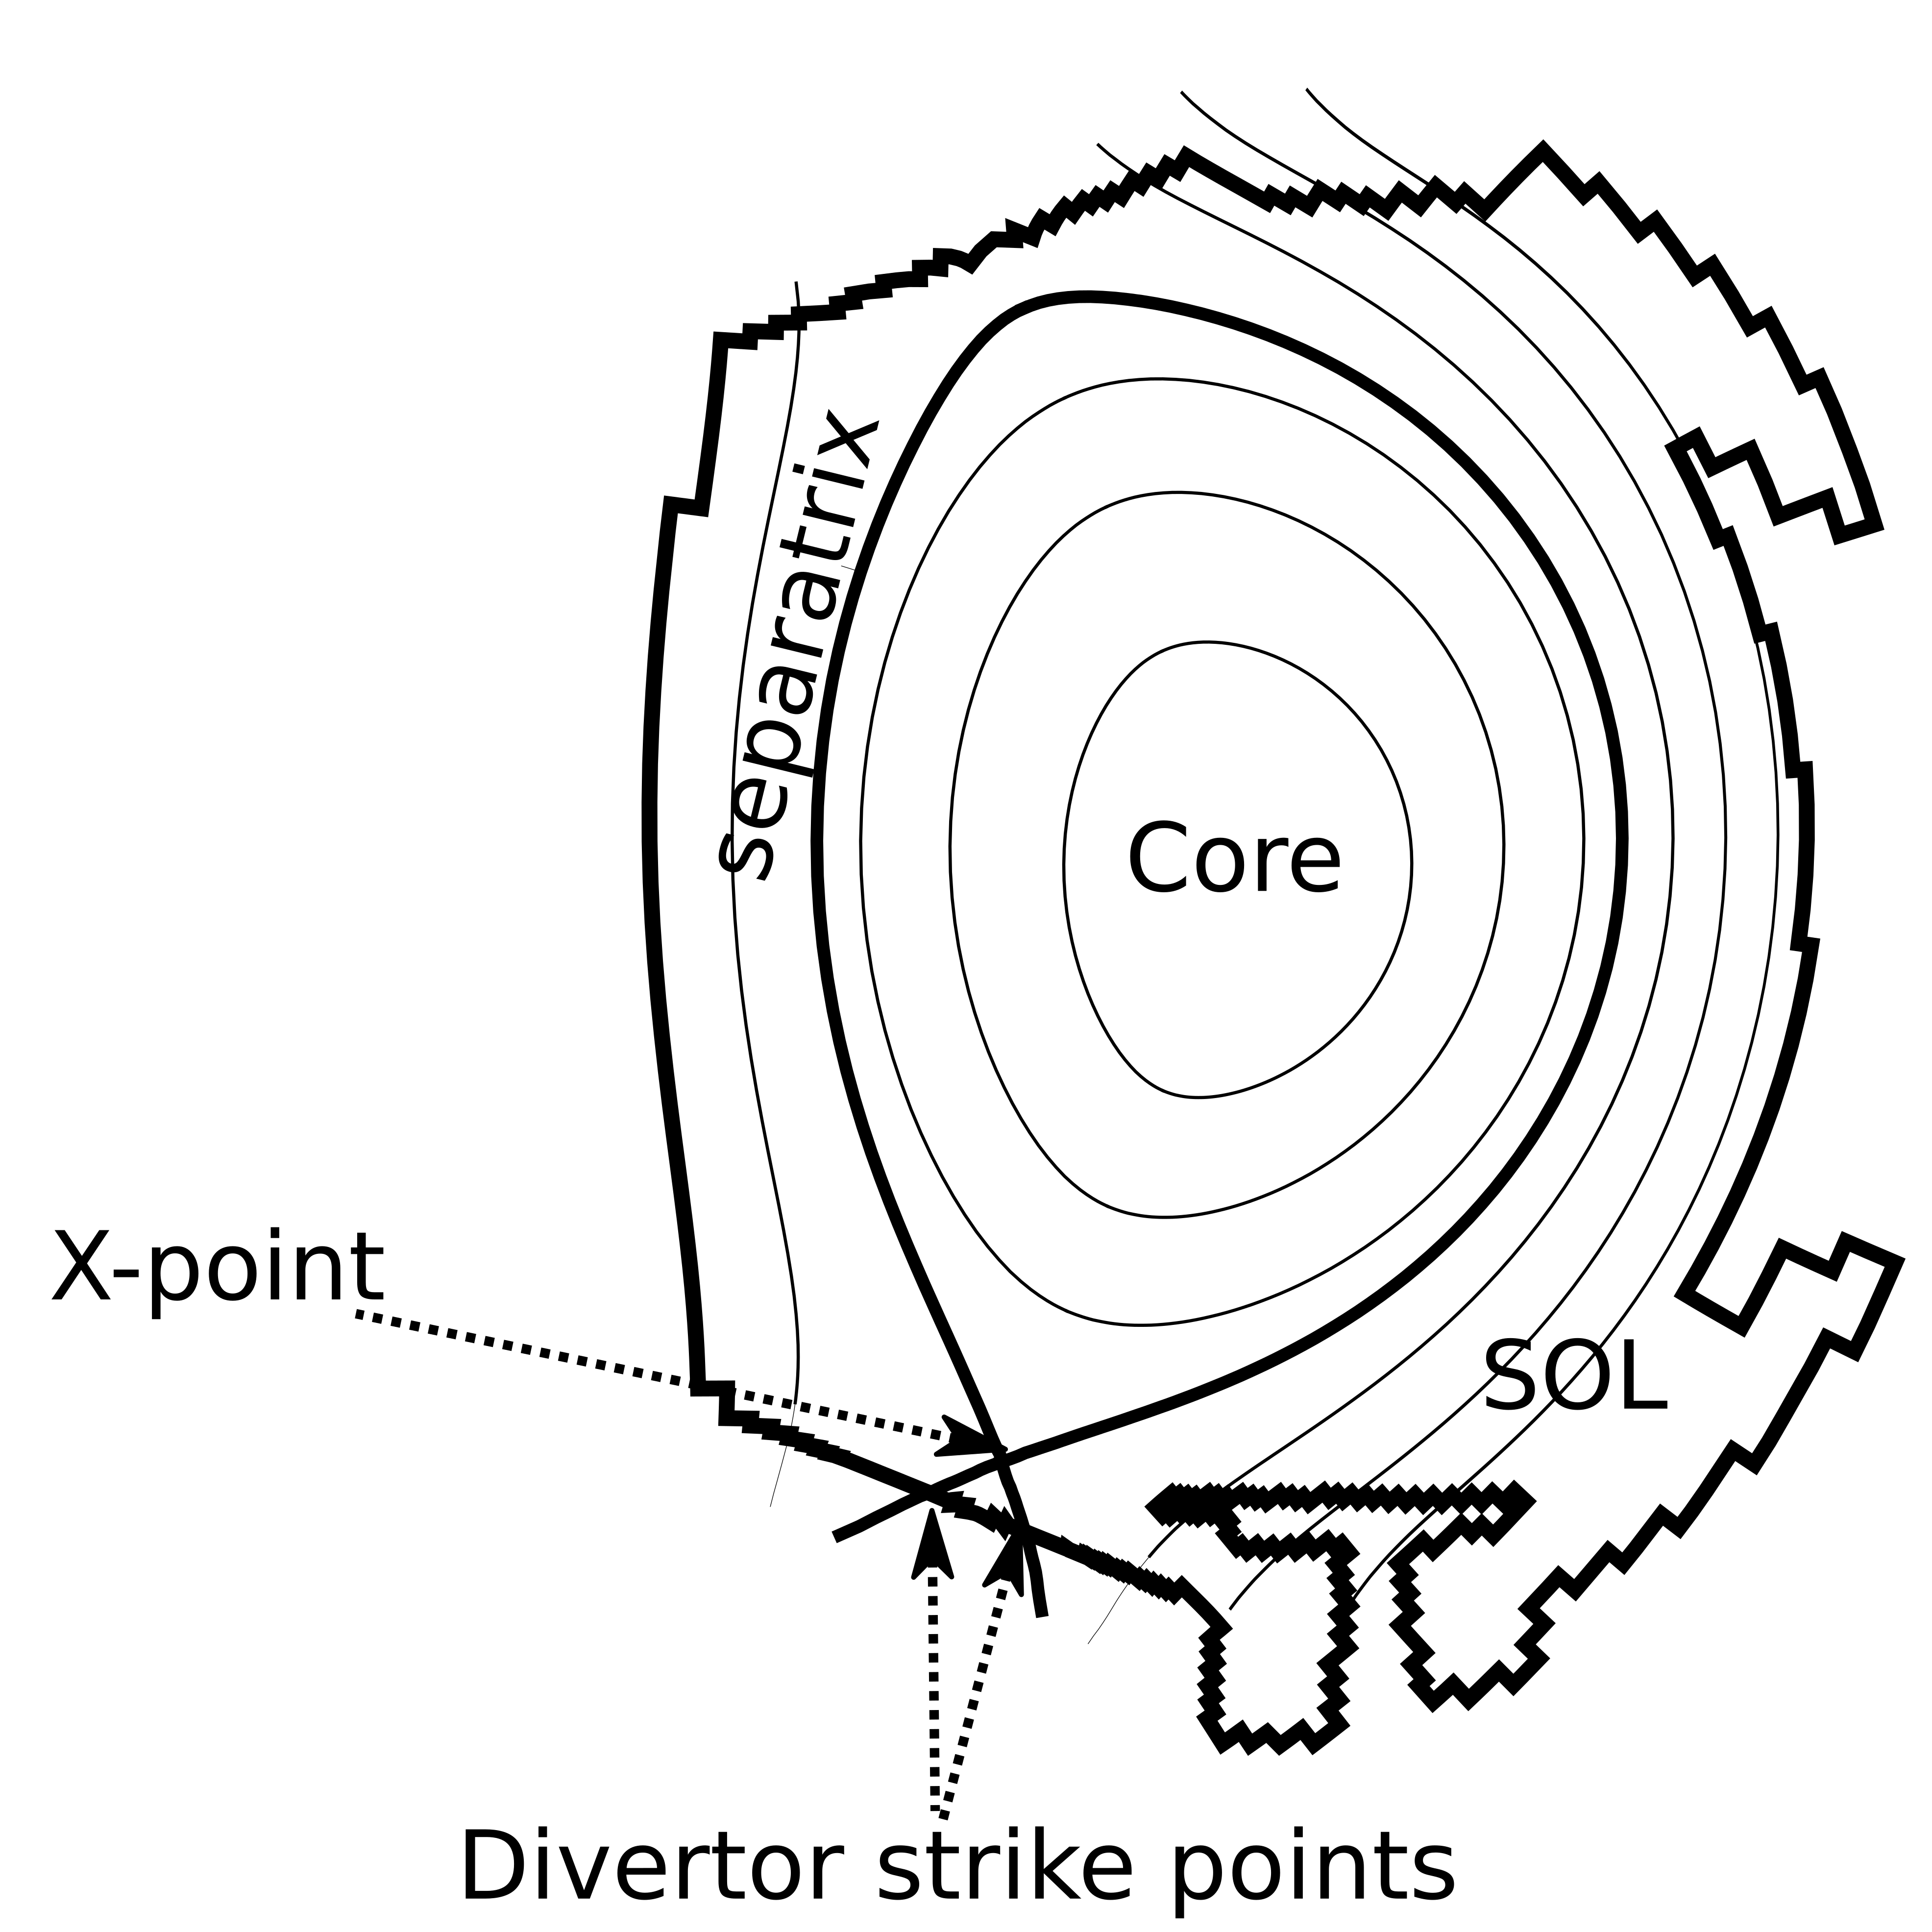
\includegraphics[height=60mm]{schemes/WESTdiverted.png}
		\subcaption{lower null configuration}
		\label{fig:WEST_diverted}
	\end{subfigure}
	\caption{Comparison of the limited and diverted configuration on a WEST geometry. }
	\label{fig:1_limdivConfigs}
\end{figure}



More exotic configurations are also feasible. In the double-null configuration, there are two divertor regions, typically located above and below the main plasma body. It splits heat loads on both divertor targets and can improve symmetry in power and particle exhaust. This symmetry helps in balancing the plasma dynamics and stabilizing the plasma, particularly with respect to vertical displacement events (VDEs), which are large-scale instabilities that can occur in tokamaks. Similarly, the X-point can be a higher-order singularity and split in more than four branches, spreading the heat load in several branches\cite{ryutov2008magnetic}. Such "snowflake" divertors can be achieved with an additional set of poloidal field coils in proximity to the divertor.

Another important parameter of the magnetic configuration is its triangularity. It refers to the shaping of the plasma cross-section, where the plasma boundary is not circular but has an elongated shape with triangular indentations. The degree of triangularity $\delta$ measures the extent of the indentation relative to the plasma’s minor radius. High triangularity configurations can enhance plasma stability and confinement, in particular in the edge region, by allowing for higher pressure gradients.



\section{Interaction between particles}
\label{sec:intro_particlesInteration}
So far we have seen how particles are confined in magnetic field lines. It gives only a partial picture of the physical processes that occur in a tokamak. A plasma contains positively and negatively charged particles at high energetic levels and they will inevitably interact between themselves. In Sec. \ref{ssec:intro_DebyeShielding} we look at how electrons and ions organize to form a state of quasi-neutrality, in Sec. \ref{sec:intro_collisions} we dive into the mechanisms that drive particle collisions and in Sec. \ref{ssec:intro_resistiveEffects} we conclude how collisions translate into resistive effects.

\subsection{Debye shielding}
\label{ssec:intro_DebyeShielding}
Debye shielding refers to the macroscopic phenomenon that electric fields naturally dissipate in a plasma at rest. When a charged particle is introduced into a plasma, electrons, being lighter and more responsive than ions, quickly redistribute themselves around the introduced charge. There is then a localized region of increased electron density that counteracts the introduced electric field. The characteristic length over which this electric field is significantly attenuated is known as the Debye length $\lambda_D$:
\begin{equation}
	\label{eq:1_DebyeLength}
	\lambda_D = \sqrt{\frac{\varepsilon_0T_e}{n_ee^2}}
\end{equation}

The Coulomb potential around a point charge $Q$ exponentially decreases for distances beyond the Debye length:
\begin{equation}
	\label{eq:1_CoulombPotential}
	\Phi(r) = \frac{Q}{4\pi\varepsilon_0r}e^{-r/\lambda_D}
\end{equation}

It effectively means that at scales larger than $\lambda_D$, the plasma can be considered quasi-neutral, where the electron density compensates the charge of all present ions.
\begin{equation}
	\label{eq:1_quasiNeutrality}
	n_e = \sum_{i}q_in_i
\end{equation}



\subsection{Particle collisions}
\label{sec:intro_collisions}

At scales below the Debye length, the Coulomb force
\begin{equation}
	\mathbf{F}_C = \frac{q_1q_2}{4\pi\varepsilon_0}\frac{\mathbf{r}}{\norm{\mathbf{r}}^3}
	\label{eq:1_CoulombForce}
\end{equation}
drives collisions between two particles with charges \( q_1 \) and \( q_2 \) at a distance \( \mathbf{r} = \mathbf{r}_2 - \mathbf{r}_1 \), where \( \varepsilon_0 \) is the vacuum permittivity. By Newton's first and third laws of motion, this force defines the acceleration of each particle \( m_{1/2}\frac{d^2\mathbf{r}_{1,2}}{dt^2} = \mathbf{F}_{12/21} \) and acts in opposite directions \( \mathbf{F}_{12} = -\mathbf{F}_{21} \) for the respective particles.


Following the derivation in Chapter 3 of Hutchinson et al. \cite{hutchinson2001introduction}, we can combine the two equations of motion to express the dynamics of a single particle (projectile) with position \( \mathbf{r} \) and reduced mass \( m_r = \frac{m_1m_2}{m_1 + m_2} \), that collides with a stationary second particle (target) at the origin. This description corresponds to a reference frame attached to the common center of mass. For an initial velocity \( \mathbf{v}_r \), the projectile will be deviated by the collision as represented in Fig. \ref{fig:TokamakBasics_collision}.

\begin{figure}[H]
	\centering
	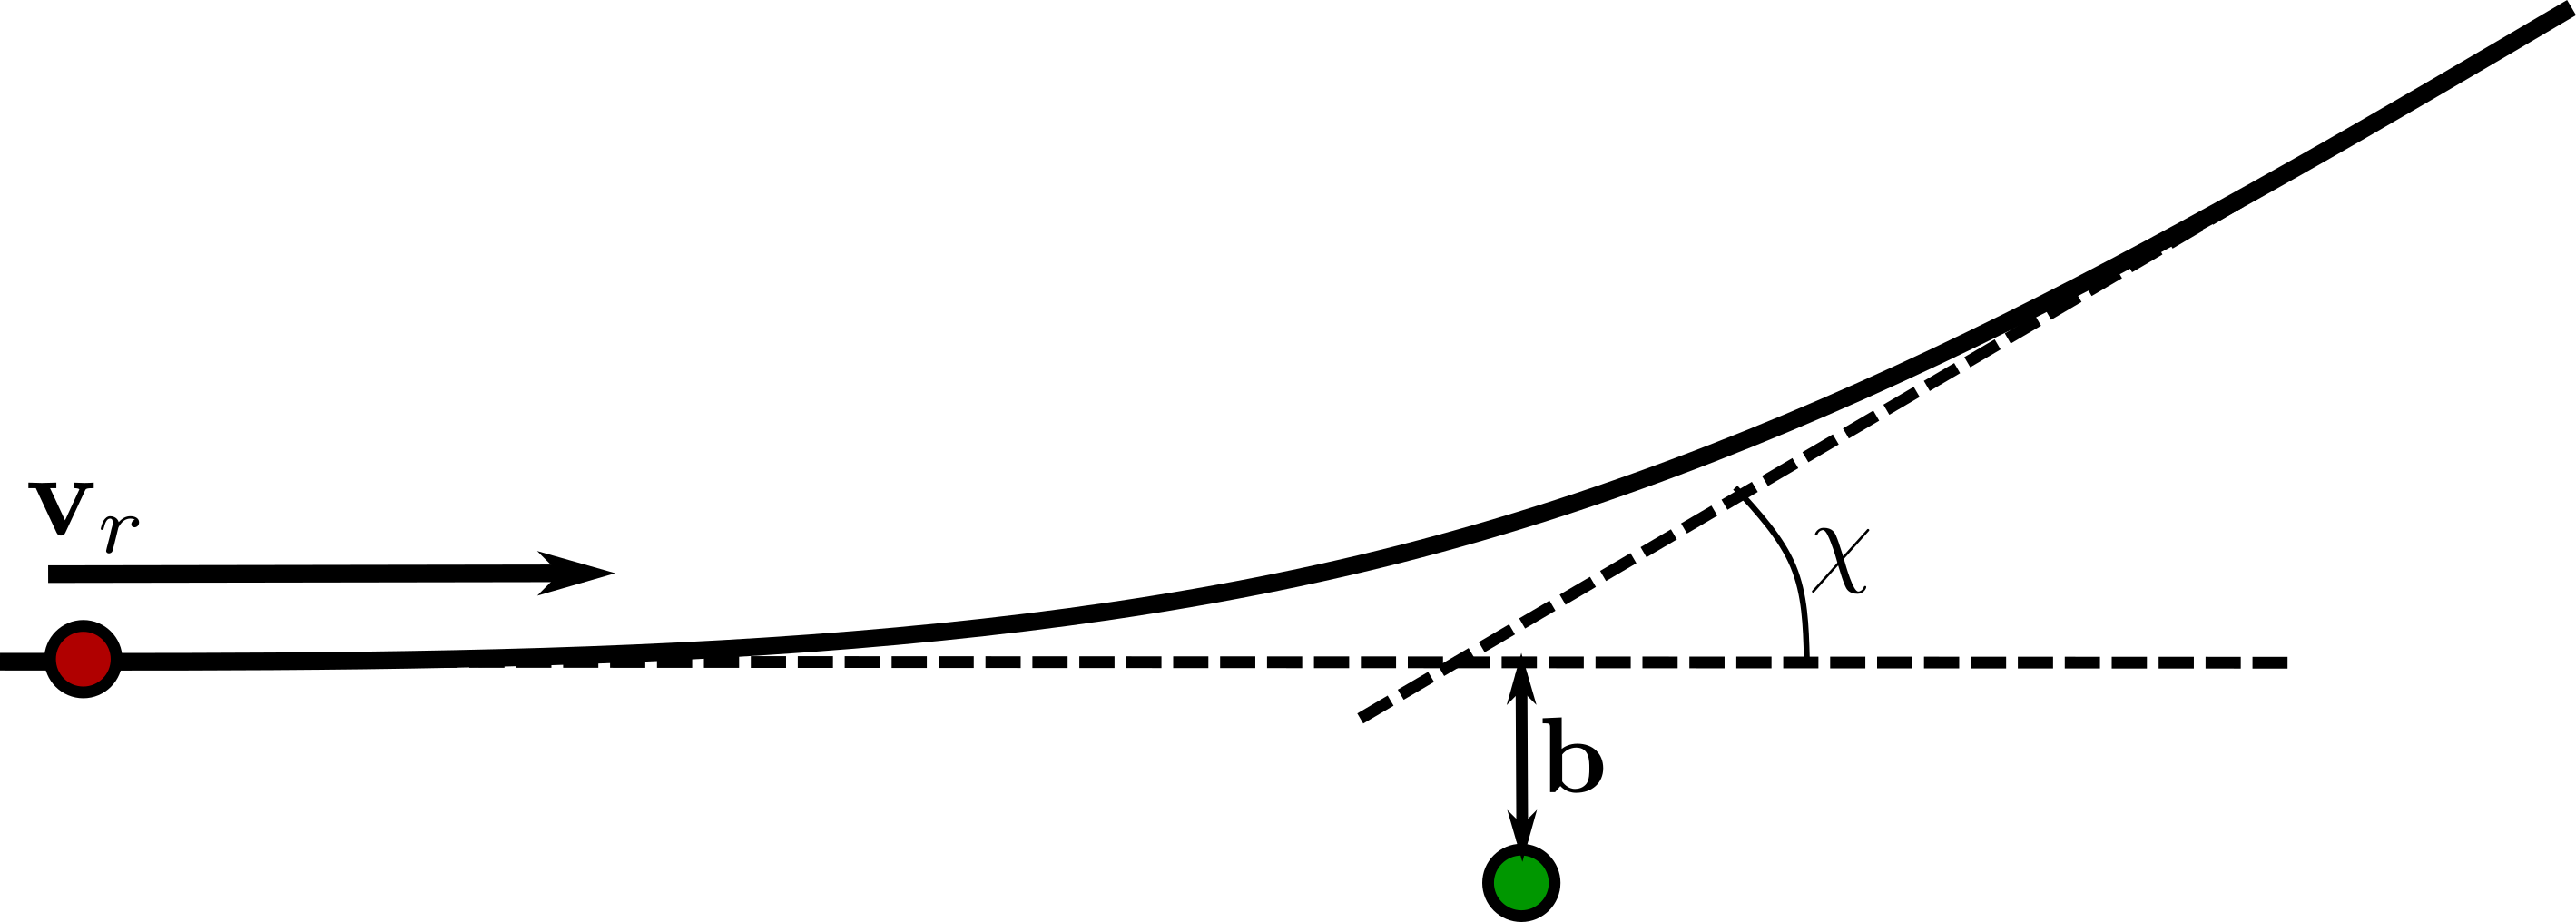
\includegraphics[width=0.62\textwidth]{schemes/collision.png}
	\caption{Trajectory of the projectile particle (red) colliding with the target particle (green). The vector \( \mathbf{b} \) denotes the impact factor and \( \chi \) is the deflection angle caused by the collision.}
	\label{fig:TokamakBasics_collision}
\end{figure}

To conserve angular momentum, the deflection of the projectile depends on the impact factor or the distance \( b = \norm{\mathbf{b}} \) of the initial trajectory to the target. Let
\begin{equation}
	b_{90} = \frac{q_1q_2}{4\pi\varepsilon_0}\frac{1}{m_r\norm{\mathbf{v}_r}^2}
\end{equation}
be the impact factor at which the projectile is deflected by a 90° angle. We can then express the deflection angle \( \chi \) at a given \( b \):
\begin{equation}
	\label{eq:1_b90}
	\chi = \tan^{-1}\frac{b_{90}}{b}
\end{equation}

This angle represents the deflection of the particle relative to the common center of mass. If we now consider two individual particles with finite mass, where the projectile approaches a stationary target with velocity \( \mathbf{v}_1 = (v_1, 0)^T \), the deflection observed in an external frame is approximately \( \chi_1 \approx \frac{m_2}{m_1 + m_2}\chi \) (using the small angle approximation). To conserve momentum in the initial direction, the target also starts moving. The projectile exits the collision with:
\begin{equation}
	\mathbf{v}'_1 = \begin{pmatrix}
		\frac{m_1v_1}{m_1 + m_2} + \frac{m_2v_1}{m_1 + m_2}\cos\chi \\
		\frac{m_2v_1}{m_1 + m_2}\sin\chi
	\end{pmatrix}
\end{equation}

At each collision, kinetic energy is transferred, and the projectile loses:
\begin{align}
	\Delta K &= K - K' = \frac{1}{2} m_1 \norm{\mathbf{v}_1}^2 - \frac{1}{2} m_1 \norm{\mathbf{v}'_1}^2 \nonumber \\
	&= \frac{2m_1^2m_2}{(m_1 + m_2)^2} v_1^2 \sin^2\frac{\chi}{2} \nonumber \\
	&\approx \frac{2m_1^2m_2}{(m_1 + m_2)^2} v_1^2 \left(\frac{b_{90}}{b}\right)^2
	\label{eq:1_particleCollision_energyLoss}
\end{align}
where the last line uses the small angle approximation \( \chi \ll 1 \).

In practice, we do not want to study every collision but are interested in the total number of collisions a particle experiences over a given length when traversing a medium with density \( n \). For that, we consider all collisions with particles at an impact factor between \( b \) and \( b + d\!b \) over a distance \( d\!x \) (see Fig. \ref{fig:TokamakBasics_collisionCrossSection}). This means we look at the volume \( V = 2\pi b d\!b d\!x \) in which we count a total of \( nV \) collisions.

\begin{figure}[H]
	\centering
	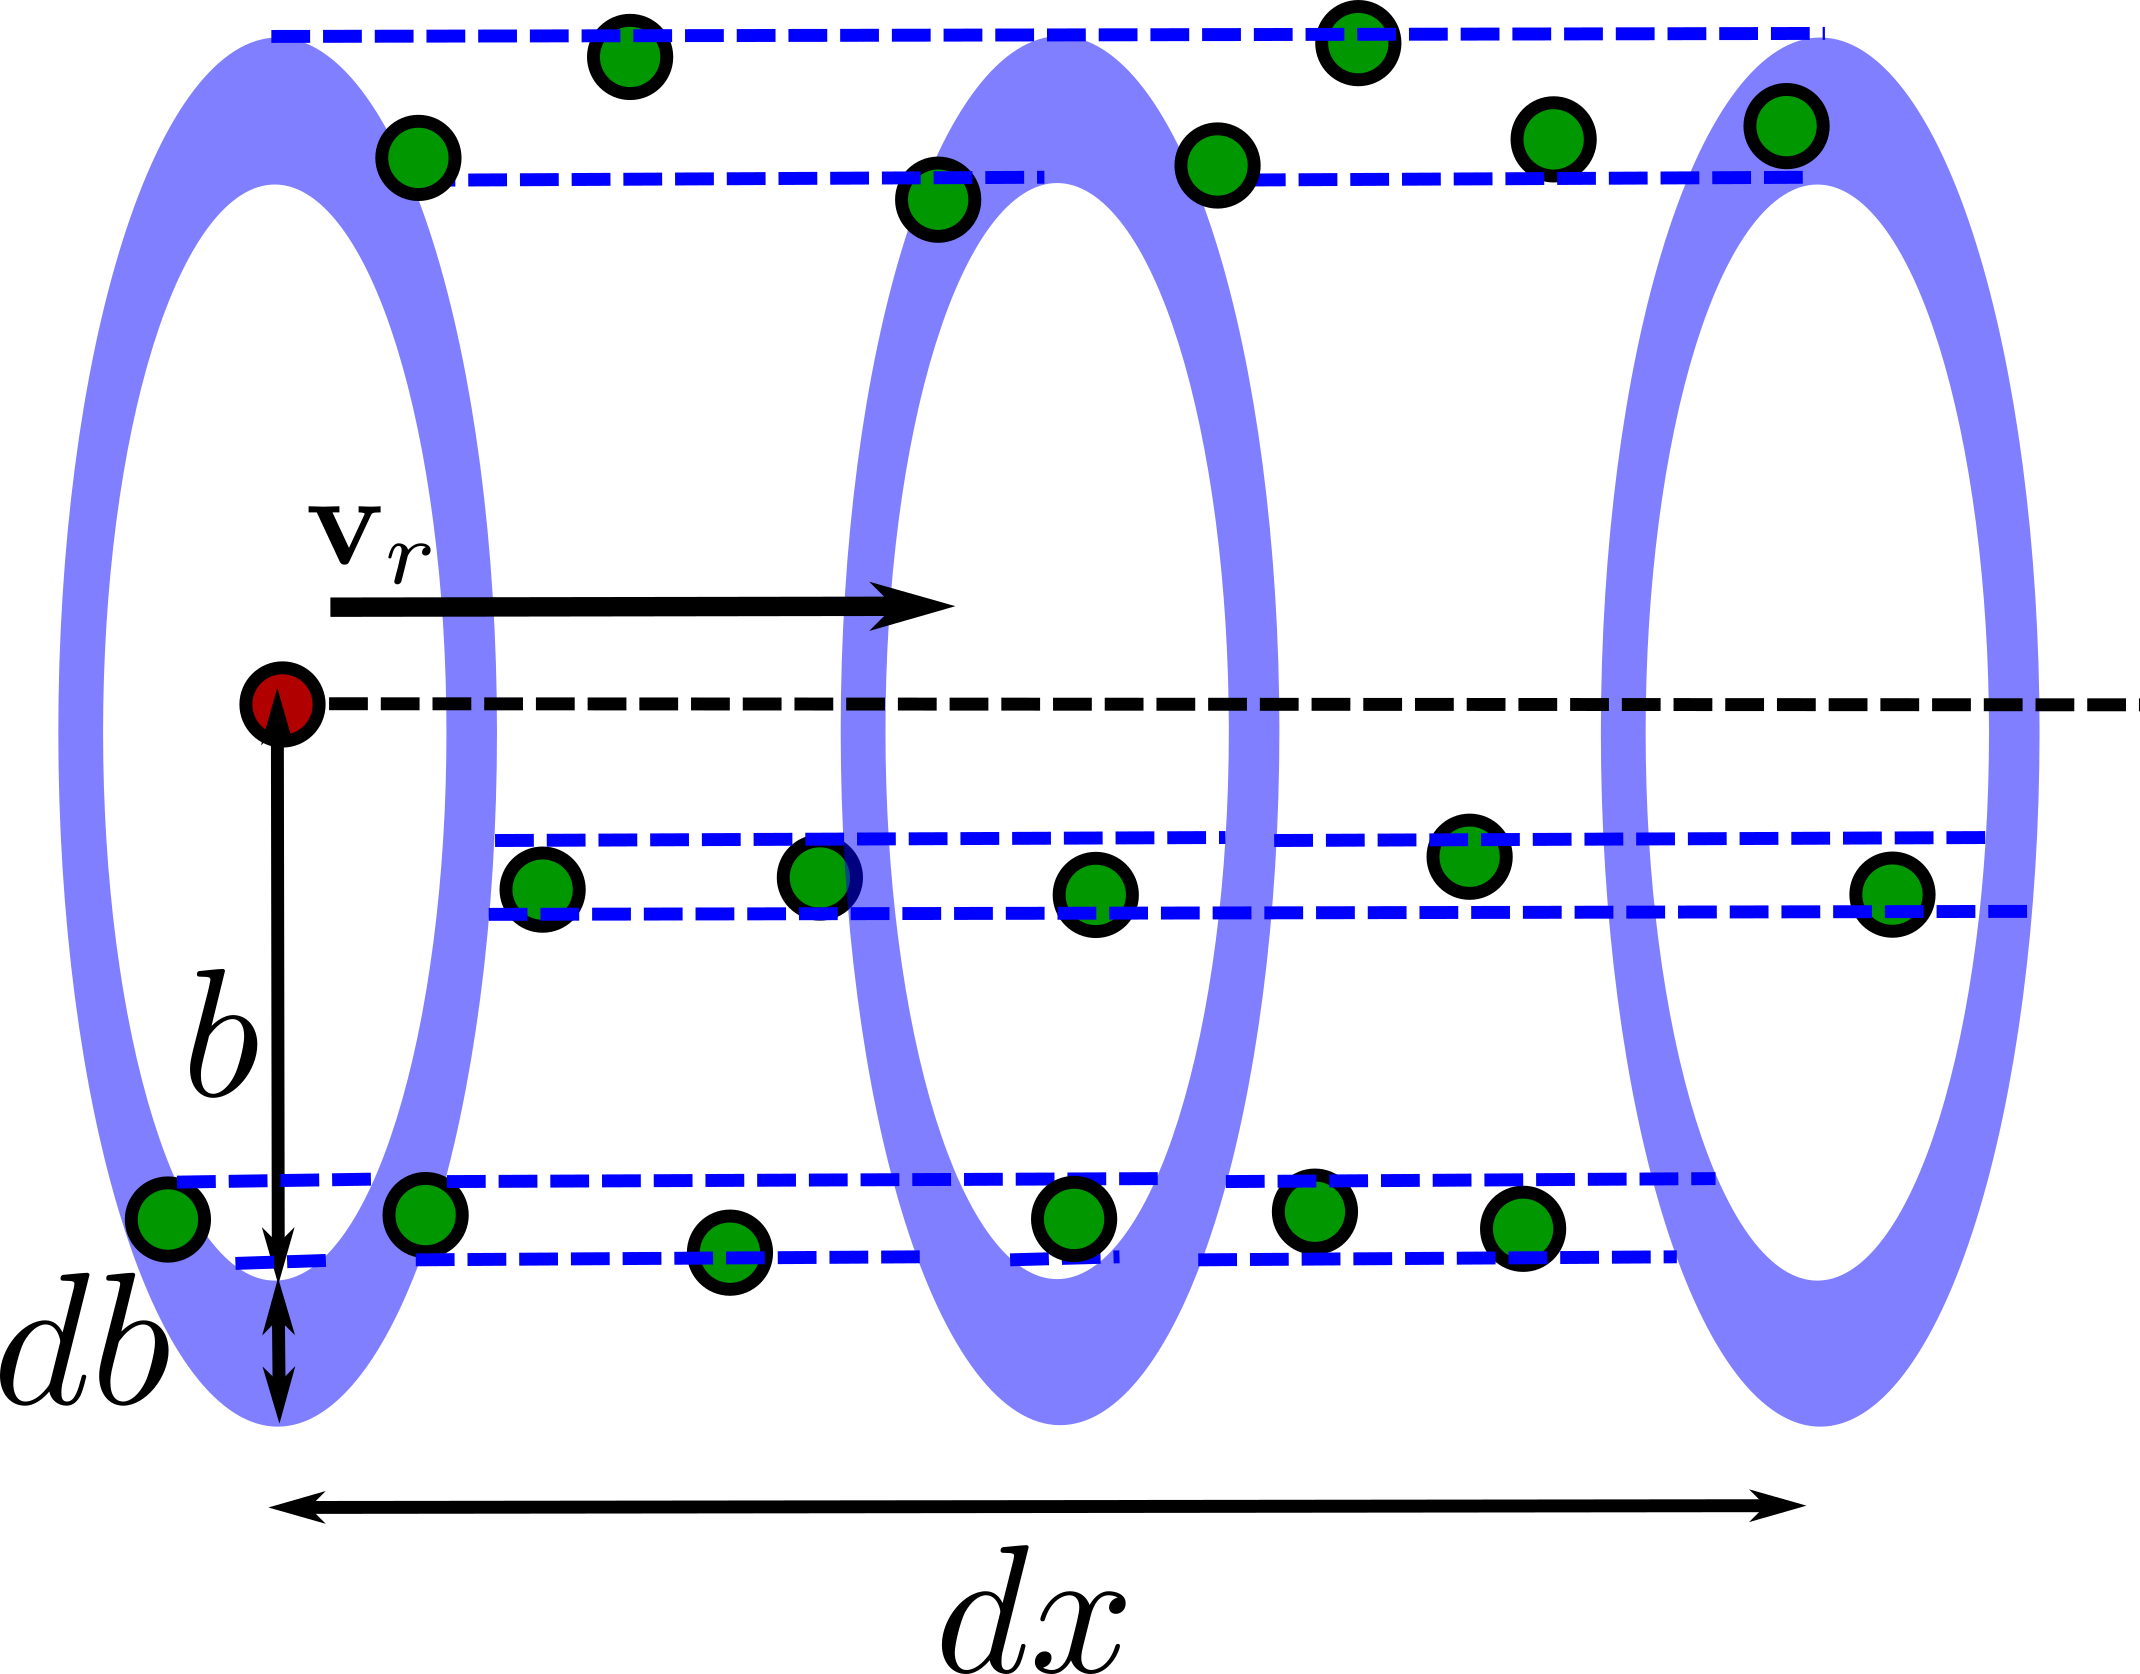
\includegraphics[width=0.45\textwidth]{schemes/collision_crossSection.png}
	\caption{Volume for given \( d\!b \) and \( d\!x \) in which collisions on the projectile are considered.}
	\label{fig:TokamakBasics_collisionCrossSection}
\end{figure}

Using Eq. \ref{eq:1_particleCollision_energyLoss} for the energy loss at each collision, we can estimate the energy our projectile loses after all collisions with the targets in the volume:
\begin{equation}
	\Delta_V K = \frac{2m_1^2m_2}{(m_1 + m_2)^2} v_1^2 \left(\frac{b_{90}}{b}\right)^2 n 2\pi b d\!b d\!x
\end{equation}

The stopping power $\frac{dK}{dx}$ describes the rate of energy loss per unit path length. It requires integrating over all possible impact factors \( b \):
\begin{equation}
	\label{eq:1_stoppingPower}
	\frac{dK}{dx} = \frac{2m_1^2m_2}{(m_1 + m_2)^2} v_1^2 n 2\pi b_{90}^2 \int_{b_{min}}^{b_{max}} \frac{1}{b} d\!b
\end{equation}

This integral diverges in both limits \( b_{min} \to 0 \) and \( b_{max} \to \infty \). We need to define cut-off values:

\begin{itemize}
	\item $b_{min} = b_{90}$ because the small angle approximation in Eq. \ref{eq:1_particleCollision_energyLoss} implies that $b>b_{90}$ \\
	\item $b_{max} = \lambda_D$ because the Coulomb potential from Eq. \ref{eq:1_CoulombPotential} vanishes quickly at distances beyond the Debye length and so does the effective Coulomb force $\mathbf{F}_C$
\end{itemize}

With these bounds, we evaluate the integral and define the Coulomb logarithm:
\begin{equation}
	\label{eq:1_CoulombLogarithm}
	\ln\Lambda = \int_{b_{90}}^{\lambda_D} \frac{1}{b} d\!b = \ln(\sqrt{\frac{\varepsilon_0T_e}{n_ee^2}}) - \ln(\frac{q_1q_2}{4\pi\varepsilon_0}\frac{1}{m_r\norm{\mathbf{v}_r}^2})
\end{equation}

For ion-ion collisions, masses $m_1 = m_2$ and charges $q_1 = q_2$ are equal. The collision frequency $\omega_c$ describes at which rate a particle loses energy through collisions relative to its total energy. The power loss is proportional to the stopping power with the particle velocity $\frac{dK}{dt} = v\frac{dK}{dx}$. We can then relate $\omega_c$ to the stopping power:

\begin{equation}
		\omega_c = \frac{v}{K}\frac{dK}{dx}
\end{equation}

If we now inject Eqs. \ref{eq:1_b90}, \ref{eq:1_stoppingPower} and \ref{eq:1_CoulombLogarithm} we obtain following expression for $\omega_c$:

\begin{align}
%	&= \frac{v}{K}\frac{2m_1^2m_2}{(m_1 + m_2)^2} v_1^2 n 2\pi b_{90}^2 \ln\Lambda \nonumber \\
%	&= \frac{v}{K}\frac{2m^2m}{(m + m)^2} v^2 n 2\pi \left(\frac{q_1q_2}{4\pi\varepsilon_0}\frac{1}{mv^2}\right)^2 \ln\Lambda \nonumber \\
%	&= \frac{vv^2 2m^3 n 2\pi }{4m^2 K} \frac{q^4}{16\pi^2\varepsilon_0^2m^2v^4}\ln\Lambda \nonumber \\
%	&= \frac{q^4 n }{16\pi m v K \varepsilon_0^2}\ln\Lambda \nonumber \\
	\omega_c&= \frac{q^4 n}{16\pi \varepsilon_0^2 \sqrt{2m}K^{3/2}}\ln\Lambda \label{eq:1_collisionFrequency}
\end{align}
Assuming that the kinetic energy follows directly the plasma temperature with the relation $K = 3/2T$, we can express the characteristic collision time $\tau_c$ and mean free path $\lambda_c$:
\begin{align}
%	\tau_c &= \frac{1}{\omega_c} = \frac{16\pi \varepsilon_0^2 \sqrt{2m}(3/2T)^{3/2}}{q^4 n \ln\Lambda} 	\nonumber \\
	\tau_c = \frac{1}{\omega_c} &= \frac{52\sqrt{3}\pi \varepsilon_0^2\sqrt{m}}{q^4 \ln\Lambda} \frac{T^{3/2}}{n}\label{eq:1_collisionTime} \\
%	\lambda_c &= \frac{v}{\omega_c} = \frac{16\pi \varepsilon_0^2 \sqrt{2m}vT^{3/2}}{q^4 n \ln\Lambda} \nonumber \\
%	&= \frac{16\pi \varepsilon_0^2 \sqrt{2m}(2K/m)^{1/2}T^{3/2}}{q^4 n \ln\Lambda} \nonumber \\
%	&= \frac{32\pi \varepsilon_0^2 (K)^{1/2}T^{3/2}}{q^4 n \ln\Lambda} \nonumber \\
%	&= \frac{32\pi \varepsilon_0^2 (3/2T)^{1/2}T^{3/2}}{q^4 n \ln\Lambda} \nonumber \\
	\lambda_c = \frac{v}{\omega_c} &= \frac{32 \sqrt{3/2}\pi \varepsilon_0^2}{q^4 \ln\Lambda}\frac{T^2}{n} \label{eq:1_meanFreePath}
\end{align}

It is worth noting that $\tau_c$ is proportional to $T^{3/2}/n$ and $\lambda_c$ to $T^2/n$ as all other terms are near-constant for a given ion in a tokamak.


\subsection{Macroscopic effects of plasma collisions}

!!!!!!!!!!!

Spitzer-Härm model: \\

Shortly state viscosity, heat resistivity and electric resistivity ! 

!!!!!!!!!!!




\section{Scrape-Off-Layer}
\label{sec:intro_SOL}

!!!!!!
Add Intro 
!!!!!!


\subsection{Fundamental sheath physics}
\label{sec:intro_sheath}

The SOL is characterized by open flux surfaces and where magnetic field lines cross the wall, the quasi-neutrality assumption from Sec. \ref{ssec:intro_DebyeShielding} does not hold anymore. The much lighter electrons travel much faster towards the wall (about $\sqrt{m_i/m_e}$ faster than ions), creating a net negative charge in the direct proximity to the wall. It is not until a few Debye lengths $\lambda_D$ before shielding restores known plasma conditions forming a region known as "electrostatic sheath". The negative charge attracts ions and repulses electrons, and we can assume that the electron density decreases exponentially approaching the wall. This eventually leads to the Bohm criterion\cite{riemann1991bohm}, which states that at the sheath entrance the ion speed must be equal or larger than the sound speed of the plasma.

\begin{equation}
	\label{eq:intro_BohmCriterion}
	v_{se} \ge c_s = \sqrt{\frac{T_i+T_e}{m_i}}
\end{equation}

From there, it is possible to calculate a sheath particle flux:
\begin{equation}
	\gamma_{se} = nv_{se}
\end{equation}

and a heat flux:

\begin{equation}
	q_{se} = \gamma n T \gamma_{se}
\end{equation}
with the sheath transmission coefficient $\gamma$. As the sheath is not collisional, these coefficients have to be determined from kinetic theory\cite{Stangeby_2000}. For hydrogen plasma, it is common to take the values $\gamma_i = 2.5$ for ions and $\gamma_e = 4.5$ for electrons.




\subsection{Confinement characteristics}
An important metric for the confinement quality is the ratio $\beta$ of plasma pressure over magnetic pressure.
\begin{equation}
	\label{eq:PlasmaBeta}
	\beta = \frac{p}{p_{mag}} = \frac{neT}{B^2/2\mu_0}
\end{equation}
There is a concurrent dynamic between thermodynamic and magnetic pressures: the former exerts an expansive force on the plasma, while the latter seeks to confine the plasma particles within their magnetic flux surfaces. A lower value of $\beta$ is generally desired for a more effective plasma confinement, but requires strong magnetic fields. However, generating such intense magnetic fields entails considerable costs and technical challenges. $\beta$ typically takes values between 1\% and 5\% in present large tokamaks. 

It is possible to distinguish between two operational regimes: L-mode and H-mode. The (L)ow-confinement mode is the standard operational mode. The plasma loses much of its energy to the wall with a consequent short confinement time. In 1982, the (H)igh-confinement mode was first observed on ASDEX in Germany and subsequently thoroughly investigated\cite{asdex1989h}. Its key feature is a strong reduction of turbulence around the separatrix, which reduces particle transport from the core to the SOL. As a consequence, temperature and density gradients steepen, forming a "pedestal" and creating a transport barrier. 

\subsection{Problematic of heat exhaust}

An important part of the heat produced in a tokamak, whether it originates from external heating or from the fusion reaction, is evacuated by hot plasma particles. Cross-field transport allows confined particles from the hot core to cross the separatrix. As they enter the SOL, they follow the magnetic field lines until they impact the divertor on the thin target band. This region is extremely critical as large amounts of power are directed on a fairly small area. It is projected for ITER that heat loads at the targets are very close to material limits\cite{gunn2017surface}. The peak heat flux $q_{peak}$ could reach values over $10MW/m^2$. For a safe tokamak operation, it is essential to well understand and predict heat fluxes on the strike points. An important metric to take into the consideration is the heat flux o power fall-off width $\lambda_q$. It describes the spread of the heat flux on the divertor targets, and a larger value allows to spread the power exhaust on a larger area. It allows to describe the heat flux at a distance $r$ from the target:

\begin{equation}
	q(r) =  q_{peak}e^{-\frac{r}{\lambda_q}}
\end{equation}

Eich et al.\cite{eich2013scaling} developed a scaling law to estimate $\lambda_q$ for H-mode operation based on machine parameters. It states that the width is inversely proportional to the toroidal magnetic field $\lambda_q\propto B_\varphi^{-0.8}$, meaning that larger machines with stronger coils will also have a thinner target line. 






